\begin{prob}
    Compute the minimum spanning tree for the following graph using Kruskal's algorithm. (Also compute the MST using Prim's algorithm and compare the results.)
    \begin{center}
        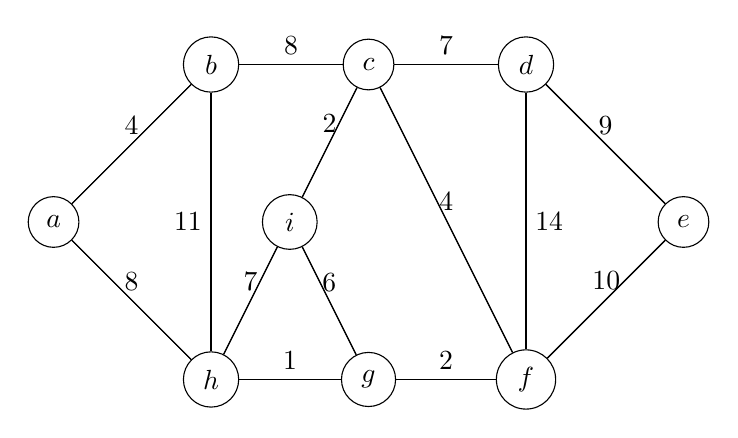
\begin{tikzpicture}
            \tikzset{
                vertex/.style={draw, circle, text width=8, align=center}, arc/.style={-}
            }
            
            \draw node[vertex] (a) at (0,0) {$a$};
            \draw node[vertex] (b) at (2,2) {$b$};
            \draw node[vertex] (c) at (4,2) {$c$};
            \draw node[vertex] (d) at (6,2) {$d$};
            \draw node[vertex] (e) at (8,0) {$e$};
            \draw node[vertex] (f) at (6,-2) {$f$};		
            \draw node[vertex] (g) at (4,-2) {$g$};
            \draw node[vertex] (h) at (2,-2) {$h$};		
            \draw node[vertex] (i) at (3,0) {$i$};		
            \foreach \x/\y in {%
                a/b, b/c,c/d,d/e,e/f,f/g,g/h,a/h,b/h,i/c,i/g,i/h,f/c,f/d%
            }{
            \draw (\x) edge[arc] (\y);
            }
            \draw[-] (a) -- node[above] {4} (b);
            \draw (a) node[right=40pt] {11} (i);
            \draw[-] (b) -- node[above] {8} (c);
            \draw[-] (c) -- node[above] {7} (d);
            \draw[-] (d) -- node[above] {9} (e);
            \draw[-] (e) -- node[above] {10} (f);
            \draw[-] (c) -- node[above] {4} (f);
            \draw[-] (g) -- node[above] {2} (f);
            \draw[-] (i) -- node[above] {6} (g);
            \draw[-] (i) -- node[above] {2} (c);
            \draw[-] (i) -- node[above] {7} (h);
            \draw[-] (g) -- node[above] {1} (h);
            \draw[-] (a) -- node[above] {8} (h);
            \draw (e) node[left=40pt] {14} (i);
        \end{tikzpicture}
    \end{center}

    \begin{responsebox}{3in}
       
        \begin{center}
            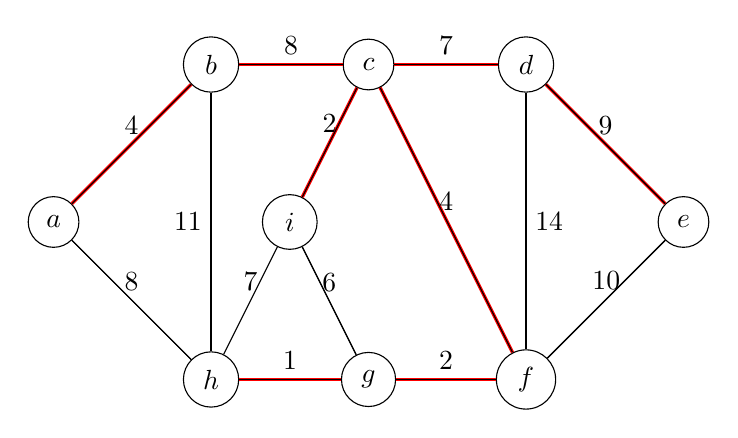
\begin{tikzpicture}
                \tikzset{
                    vertex/.style={draw, circle, text width=8, align=center}, arc/.style={-}
                }
                
                \draw node[vertex] (a) at (0,0) {$a$};
                \draw node[vertex] (b) at (2,2) {$b$};
                \draw node[vertex] (c) at (4,2) {$c$};
                \draw node[vertex] (d) at (6,2) {$d$};
                \draw node[vertex] (e) at (8,0) {$e$};
                \draw node[vertex] (f) at (6,-2) {$f$};		
                \draw node[vertex] (g) at (4,-2) {$g$};
                \draw node[vertex] (h) at (2,-2) {$h$};		
                \draw node[vertex] (i) at (3,0) {$i$};		
                \foreach \x/\y in {%
                    e/f,g/h,a/h,b/h,i/g,f/d%
                }{
                \draw (\x) edge[arc] (\y);
                }
                \foreach \x/\y in {%
                    a/b, b/c,c/d,d/e,f/g,i/c,g/h,f/c%
                }{
                \draw (\x) edge[very thick, red, -] (\y);
                }
                \draw[-] (a) -- node[above] {4} (b);
                \draw (a) node[right=40pt] {11} (i);
                \draw[-] (b) -- node[above] {8} (c);
                \draw[-] (c) -- node[above] {7} (d);
                \draw[-] (d) -- node[above] {9} (e);
                \draw[-] (e) -- node[above] {10} (f);
                \draw[-] (c) -- node[above] {4} (f);
                \draw[-] (g) -- node[above] {2} (f);
                \draw[-] (i) -- node[above] {6} (g);
                \draw[-] (i) -- node[above] {2} (c);
                \draw[-] (i) -- node[above] {7} (h);
                \draw[-] (g) -- node[above] {1} (h);
                \draw[-] (a) -- node[above] {8} (h);
                \draw (e) node[left=40pt] {14} (i);
            \end{tikzpicture}
        \end{center}
    \end{responsebox}   
\end{prob}
